\section{Experimentos y análisis de resultados}
	
	\subsection{Procedimiento de desarrollo de la práctica}
	
	\paragraph{}Para realizar la práctica, se ha optado por implementar las heurísticas propuestas en el lenguaje de programación \textsc{Java}. El ejecutable que se entrega junto a este documento ha sido compilado bajo \textsc{ Apache NetBeansIDE 12.0}.
	
	\subsubsection{Equipo de pruebas}
	
	\paragraph{}Los resultados de las heurísticas han sido obtenidos en el siguiente equipo:
	
		\begin{itemize}
			
			\item Host:
			\item S.O:
			\item Kernel:
			\item CPU:
			\item GPU:
			\item GPU:
			\item Memoria RAM :
			
		\end{itemize}

	\subsubsection{Manual de usuario}
	
		\paragraph{}Para ejecutar el software asegúrese de que el archivo .jar proporcionado se ubica en el mismo directorio que la carpeta \emph{archivos}. 
		
		\paragraph{}Cuando se muestre la GUI, podrá seleccionar la heurística que desee mediante el botón correspondiente. Una vez empiece la ejecución de una heurística no sera posible seleccionar otra hasta que finalice su ejecución. Los resultados finales se mostrarán en el cuadro de texto, a su vez, se generan los log correspondientes a cada archivo y semilla en la carpeta Log.
	
		\begin{figure}[H]
		
			\centering
			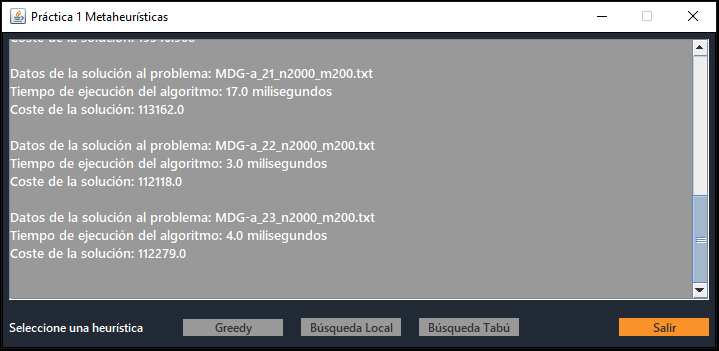
\includegraphics[scale=0.4]{img/GUI}
			\caption{GUI}
		
		\end{figure}
	
	\subsection{Parámetros de los algoritmos}
	
		\subsubsection{Sistema de Colonias de Hormigas}
		
			\begin{itemize}
				\item Iteraciones: Número de iteraciones objetivo, es una de las condiciones de parada del algoritmo, en cada iteración se generan el número
				especificado de hormigas, valor por defecto = 10000.
				\item Tmax: Tiempo máximo expresado en segundos para cada problema, es la segunda condición de parada para el algoritmo, valor = 600.
				\item Q0: Valor de la regla de transición, valor por defecto = 0,95.
				\item Beta: Valor por defecto = 1.
				\item Alfa: Valor por defecto = 1.
				\item Rho: Actualización de la feromona global, valor por defecto = 0,1.
				\item Phi: Actualización local de la feromona, valor por defecto = 0,1.
				\item Delta: Valor del parámetro para LRC, un valor más alto indica un LRC más restringida, valor por defecto 0,75.
				\item Número de hormigas: Define la cantidad de hormigas que se desarrollan en cada iteración, valor por defecto = 10.
				
				
				
				
			\end{itemize}

	
	\subsubsection{Semillas}
	
	\paragraph{}Para la generación de números pseudoaleatorios se utiliza una semilla previamente definida en el archivo de configuración, en este caso es 77356084. Esta semilla se va rotando en las 5 iteraciones de cada archivo.
	
	
	\paragraph{} 77356084 $\rightarrow$ 73560847 $\rightarrow$ 35608477  ...
	
	
	\subsection{Análisis de los resultados}
	
		\subsection{SCH con $\alpha$ = 1, $\beta$ =1}
		
		\begin{table}[H]
			\begin{center}
				\begin{tabular}{| c | c | c | c | c | c | c |}
					\hline
					\multicolumn{7}{ |c| }{SCH $\alpha$ = 1, $\beta$ =1} \\ \hline
					& \multicolumn{2}{ |c| }{GKD-c\_1\_n500\_m50} & \multicolumn{2}{ |c| }{GKD-c\_2\_n500\_m50} & \multicolumn{2}{ |c| }{GKD-c\_3\_n500\_m50} \\ \hline
					Ejecución & Coste & Tiempo & Coste & Tiempo & Coste & Tiempo \\ \hline
					1 &19485,19 & 1205,00 & 19700,36 & 1131,00 & 19547,22 & 1169,00\\
					2 &19485,19 & 1184,00 & 19701,52 & 1109,00 & 19547,22 & 1121,00\\
					3 &19485,19	& 1142,00 & 19701,52 & 1118,00 & 19547,22 & 1109,00\\
					4 &19485,19	& 1179,00 & 19701,52 & 1103,00 & 19547,22 & 1112,00\\
					5 &19485,19 & 1157,00 & 19700,36 & 1132,00 & 19547,22 & 1121,00\\ \hline
					Media & 0,00\% & 1173,40 & 0,00\% & 1118,60 & 0,00\% & 1126,40\\ \hline
					Devs. típica & 0,00\%	& 24,48 & 0,00\% & 12,93 & 0,00\% & 24,41 \\ \hline
				\end{tabular}
				\caption{Resultados GKD}
				\label{tab:tab2POINTE2GKD}
			\end{center}
		\end{table} 
		
		
		\begin{table}[H]
			\begin{center}
				\begin{tabular}{| c | c | c | c | c | c | c |}
					\hline
					\multicolumn{7}{ |c| }{SCH $\alpha$ = 1, $\beta$ =1} \\ \hline
					& \multicolumn{2}{ |c| }{SOM-b\_11\_n300\_m90} & \multicolumn{2}{ |c| }{SOM-b\_12\_n300\_m120} & \multicolumn{2}{ |c| }{SOM-b\_13\_n400\_m40} \\ \hline
					Ejecución & Coste & Tiempo & Coste & Tiempo & Coste & Tiempo\\\hline
					1 &20644,00 & 1807,00 & 35848,00 & 3839,00 & 4631,00 & 1211,00\\
					2 &20650,00	& 1752,00 & 35813,00 & 3751,00 & 4542,00 & 1054,00\\
					3 &20631,00	& 1786,00 & 35847,00 & 3449,00 & 4571,00 & 817,00\\
					4 &20674,00	& 1825,00 & 35803,00 & 3713,00 & 4614,00 & 646,00\\
					5 &20638,00 & 1800,00 & 35871,00 & 3847,00 & 4540,00 & 657,00\\\hline
					Media &-0,46\% & 1794,00 & -0,12\% & 3719,80 & -1,68\% & 877,00\\ \hline
					Devs. típica & 0,08\%	& 27,36 & 0,08\% & 161,82 & 0,89\% & 249,12 \\ \hline
				\end{tabular}
				\caption{Resultados SOM}
				\label{tab:tab2POINTE2SOM}
			\end{center}
		\end{table} 
		
		\begin{table}[H]
			\begin{center}
				\begin{tabular}{| c | c | c | c | c | c | c |}
					\hline
					\multicolumn{7}{ |c| }{SCH $\alpha$ = 1, $\beta$ =1} \\ \hline
					& \multicolumn{2}{ |c| }{MDG-a\_21\_n2000\_m200} & \multicolumn{2}{ |c| }{MDG-a\_22\_n2000\_m200} & \multicolumn{2}{ |c| }{MDG-a\_23\_n2000\_m200}\\\hline
					Ejecución & Coste & Tiempo & Coste & Tiempo & Coste & Tiempo\\\hline
					1 &112242,00 & 44907,00 & 112506,00 & 46008,00 & 111991,00 & 44417,00\\
					2 &112280,00 & 43616,00 & 112443,00	& 43669,00 & 112497,00 & 43752,00\\
					3 &111963,00 & 45431,00	& 112604,00	& 44006,00 & 111921,00 & 44011,00\\
					4 &112012,00 & 42691,00	& 112723,00	& 43679,00 & 112302,00 & 43656,00\\
					5 &112367,00 & 44207,00	& 111886,00	& 43836,00 & 112163,00 & 43111,00\\\hline
					Media &-1,83\% & 44170,40 & -1,66\% & 44239,60 & -1,71\% & 43789,40\\ \hline
					Devs. típica & 0,15\%	& 1075,76 & 0,28\% & 998,07 & 0,20\% & 480,21 \\ \hline
				\end{tabular}
				\caption{Resultados MDG}
				\label{tab:tab2POINTE2MDG}
			\end{center}
		\end{table}
		
		
		\subsection{SCH con $\alpha$ = 2, $\beta$ =1}
		
		\subsection{SCH con $\alpha$ = 1, $\beta$ =2}
	
	
